\section{FlyClient under Velvet Fork}
\label{sec:flyclient}
In the FlyClient paper~\cite{flyclient} a velvet fork is suggested for the deployment of the protocol as-is.
We now describe an explicit attack against
the FlyClient protocol under velvet fork deployment.
This is a variation of our Chainsewing Attack of Section~\ref{sec:attack}.

\subsection{The FlyClient Protocol}
	The FlyClient protocol suggests that block headers additionaly include an MMR root of all the blocks in the chain. The protocol uses this root hash in multiple ways, both for chain synchronization and specific block queries. Consider a block $b$ which is appended to the chain $\chain$ at height $h_b$:
	\begin{itemize}
		\item the prover generates a merkle inclusion proof $\Pi_b$ for the existence of $b$ at height $h_b$ in $\chain$ with respect to the MMR root included in the \emph{tip} of the stable chain $\chain[-1]$
		\item the verifier receives the merkle root of the chain from a prover and an inclusion proof $\Pi_b$ for block $b$. He also generates from $\Pi_b$ the root of the MMR subtree of all blocks in $\chain$ from genesis up to $\chain[h_b - 1]$ and verifies that it is equal to the merkle root included in the header of block $b$.
	\end{itemize}
	The above proofs are produced with respect to the MMR root included in $\chain[-1]$.

	\vspace{2mm}
	\noindent
	A high level description of the FlyClient is as follows. Consider a verifier, a superlight client, that asks to synchronize to the current longest valid chain. Suppose that he receives different proofs from two provers. Each prover sends (the header) of the last block in the chain, $\chain[-1]$, and a claim for the number of blocks in his chain, $\lvert \chain \rvert$ (which he will later be interrogated upon). If both proofs are valid, then the one claiming the greater block count is selected. The validity check of a proof goes as follows.
	The verifier has received $\chain[-1]$, $\lvert \chain \rvert$ and queries $k$ random block headers from each prover based on a specific probabilistic sampling algorithm. For each queried block $B_i$ the prover sends the header of $B_i$ along with an MMR subtree inclusion proof $\Pi_{B_i}$ that $B_i$ is the $i_\text{th}$ block in the chain. The verifier also checks that $B_i$ is normally mined on the same chain as $\chain[-1]$ by verifying that the root included in $B_i$ is the MMR root of the first ($\lvert \chain \rvert - 1$) blocks' subtree. If the $k$ random sampled blocks successfully pass through this verification procedure then the proof is considered valid, otherwise the proof is rejected by the verifier.
	The chain synchronization protocol is given in Algorithm~\ref{alg:flyclient_suffix_protocol}.

	\begin{algorithm}[h]
		\caption{\label{alg:flyclient_suffix_protocol}FlyClient suffix protocol~\cite{flyclient}}
		\begin{flushleft}
		A verifier performs the following steps speaking with two provers who want to convince him that they hold a valid chain of length $n+1$. At least one of the provers is honest. If the provers claim different lengths for their claims then the longer chain is checked first.
		\begin{enumerate}
			\item The provers send to the verifier the last block header in their chain. Each header includes the root of an MMR created over the first $n$ blocks of the corresponding chain.
			\item The verifier queries $k$ random block headers from each prover based on a probabilistic sampling algorithm~\cite{flyclient}.
			\item For each queried block, $B_i$, the prover sends the header of $B_i$ along with an MMR proof $\Pi_{B_i \in \chain}$ that $B_i$ is the $i-$th block in the chain,
					  and that $B$'s MMR contents form a prefix of the MMR included in $\chain$.
			\item The client performs the above checks for each block $B_i$ according to the previous step.
			\item The client rejects the proof if any checks fail.
			\item Otherwise, the client accepts $\chain$ as the valid chain.
		\end{enumerate}
		\end{flushleft}
	\end{algorithm}

	\begin{algorithm}[h!]
		\caption{\label{alg:flyclient_iinfix_protocol}FlyClient infix protocol~\cite{flyclient}}
		\begin{flushleft}
		The verifier queries the prover for the header and MMR proof for a single block $b$ in the prover's chain of $n+1$ blocks.
		\begin{center}
			\textbf{Verifier}
		\end{center}
		\begin{enumerate}
			\item Has the root of the MMR of $n$ blocks stored in the header of $C[-1]$
			\item Queries prover for the header of block $b$ and for $\Pi_{b \in C}$
			\item Checks the validity of the MMR inclusion proof $\Pi_{b \in C}$
			\item Checks that the MMR of $b$ has contents that are a prefix of the MMR of $C[-1]$
			\item If everything checks out, accepts the block proof
		\end{enumerate}
		\begin{center}
			\textbf{Prover}
		\end{center}
		\begin{enumerate}
			\item Has chain of $n+1$ blocks and the MMR of the first $n$ blocks
			\item Receives query for block $b$ from verifier
			\item Calculates $\Pi_{b \in C}$ from MMR$_C$
			\item Sends header of $b$ and $\Pi_{b \in C}$ to verifier
		\end{enumerate}
		\end{flushleft}
	\end{algorithm}

	Once the longest chain has been chosen, the infix validation is similar to the previous algorithm.
	The verifier is synchronized to a chain $\chain$ and already has the tip of the chain $\chain[-1]$. He then queries the prover and receives the header of the specific block of interest $B$ in $\chain$ and the inclusion proof $\Pi_{B \in \chain}$. Then the verifier checks the validity of $B$ in the same way as already described for the random sampled blocks in the synchronization protocol.
	The prover/verifier single-query protocol is given in Algorithm~\ref{alg:flyclient_iinfix_protocol}.


\subsection{Velvet MMRs}
	In a velvet fork deployment of FlyClient, upgraded miners additionally include an MMR root in each block's header.
    The claim made in the paper is that considering a constant fraction $\alpha$ of upgraded blocks in the chain, an honest prover could produce proofs
    by utilizing only these blocks and by joining the intermediary blocks together.
    The claim is that the velvet proofs remain secure. The velvet protocol is susceptible to a chainsewing attack, succeeding with non-negligible probability.
    We now give a high-level overview of this attack.

	Velvet fork requires any block to be accepted in the chain regardless the validity of the auxiliary data coming with the protocol update.
    In the case of FlyClient, an adversary may produce blocks which are compatible to the basic consensus rules but contain invalid MMR information.
    As an example, consider an invalid MMR that omits blocks existing in $\chain$ or contain blocks which belong in temporary forks of $\chain$.
    We call adversarially generated blocks containing invalid MMRs \emph{thorny} blocks.

\subsection{The Attack}
	Consider the security impact of thorny blocks in the FlyClient protocol.
	Due to the velvet FlyClient description being only partial, we make
	make a couple of assumptions considering how thorny blocks are treated by the protocol.

	When an upgraded \emph{miner} creates a new block, he must include an MMR in this block
	pointing to all previous blocks (thorny or not).

	When the verifier receives two FlyClient client proofs, he will see two chain tips $C_\mathcal{A}[-1]$ (by the adversary) and $C_B[-1]$
	(by the honest prover). The honest tip $C_B[-1]$ will be a non-thorny block, while the block $C_\mathcal{A}[-1]$ may be thorny or
	non-thorny. He then interrogates each of the provers. During the interrogation, each block $b$ sampled by the verifier may
	contain their own MMR. In case $b$ does not contain an MMR ($b$ is an unupgraded block), the verifier cannot check consistency
	between $b$ and $C[-1]$.
	In the case of the honest prover, it is possible that the sampling yields a block $b$ which is upgraded but thorny.
	In this case, the consistency check between $b$ and $C_B[-1]$ will fail.
	Similarly, in the case of the adversarial consistency check, the consistency check may succeed in case both $b$ and $C_\mathcal{A}[-1]$
	even if both of these are thorny.

	In case the honest verifier readily rejects a proof with any inconsistency, as in the soft fork case, the adversary can easily make any honest proof fail
	by simply introducing thorny blocks in the chain. Therefore, the verifier must accept that some consistency check between $b$ and $C[-1]$ will fail.
	On the other hand, the verifier cannot allow any number of inconsinstencies freely. To see why,
	consider the following attack. Let the honest chain have three consecutive blocks $b_i$, $b_{i+1}, b_{i+2}$ at heights $i, i+1, i+2$ respectively. The attacker produces a thorny block $b'_{i+1}$ on top of $b_i$ containing a double spend transaction in conflict with $b_{i+1}$.
	Whenever she wants to convince the verifier that the honest chain contains $b'_{i+1}$ she produces another thorny block $b_j$ on top of the current chain's tip and sends her proof (setting $C_\mathcal{A}[-1] = b_j$). Note that $b_j$ is a thorny block that contains an MMR that includes
	$b'_{i+1}$. The adversary claims that $b'_{i+1}$ and $b_j$ are the only non-thorny blocks in the chain, contrary to reality, where all \emph{other} upgraded blocks are non-thorny.
	More specifically $b_j$ will appear in the proof as it is the tip of the chain, while $b_{i+1}$ will be in the proof
	only if it is selected by the random sampler. Her proof will only be found invalid if the random sampler queries both blocks at heights $i+1, i+2$, so that the invalid prevId pointer shows up. The attacker can decrease this probability
	by letting the chain grow enough before attempting to construct a proof, as the random sampler chooses older blocks with lower probability (the probability of this sampling occuring is negligible if the proof size is logarithmic). When the verifier receives two valid proofs of the same length, one from the attacker and one from an honest node,
	the verifier cannot tell which proof is the correct one. One mechanism to avoid this attack is to have the verifier perform consistency verification and count how many of
	these verifications are successful. In the case of the above attack, most upgraded blocks will appear inconsistent with the claimed (thorny) tip.
	Intuitively, under an appropriate velvet honest majority assumption, and for sufficiently long underlying chains, the honest proof (ending in a non-thorny block)
	will pass more consistency checks among the samples performed
	by the verifier, as compared to the adversarial proof (ending in a thorny block).

	We conclude that an appropriately designed velvet variant of the FlyClient protocol must allow for inconsistencies, but must compare proofs depending on how many
	consistency checks pass. Despite this favourable version of the FlyClient protocol, we give a sketch of a chainsewing attack which works
	with an adversary that has more than $1/3$ mining power and a constant proportion of the honest upgraded parties (despite the claimed $1/2$ adversarial bound in the FlyClient work) .

	The adversary utilizes more than one thorny blocks, in order to cut-and-paste portions from the chain adopted by honest parties to her fork chain.
    The adversary acts as follows.
		She initially creates a transaction in an honest block $b$. She subsequently forks from the parent of $b$ to create a block $b'$ containing
		a double spend.
    Afterwards she mines block $a'$ in the honest chain $\chain_B$, which includes an MMR root containing $b'$.
    Next she keeps mining blocks on top of the honest chain, ensuring that they contain MMR commitments to
		$a'$, $b'$ and the whole other honest chain, excluding $b$.
    Additionally, during this period when she mines on $\chain_B$ she tries to suppress any honest upgraded block in $\chain_B$ by mining selfishly.
    When an honest upgraded block $\chain[i]$ is appended she mines on top of block $\chain[i-1]$.
    Even if she mines a block and the suppression fails she can still use her fresh block in her proof by continuing to construct consistent MMRs
    in the coming blocks as described before.
		Figure~\ref{fig:combined_chainsewing_flyclient} illustrates an example of the underlying suppression attack.
    At some point, the adversary produces her proof.
    From the verifier's perspective the black colored blocks form a valid chain,
    since the tip contains consistent MMR commitments with all these blocks.
    In addition, the random sampling performed by the FlyClient protocol will favour the adversary
		(with the exception of the case where a consecutive thorny and honest blocks are sampled).
		We conclude that the FlyClient protocol may be possible to work in velvet conditions through this construction,
		but similar assumptions to our construction in Section~\ref{sec:construction} will be necessary to avoid such suppression attacks.
		Therefore, a stronger velvet honest majority assumption is required.

	\begin{figure}
		\begin{center}
			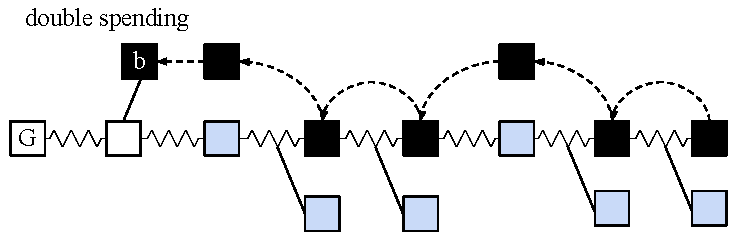
\includegraphics[width=0.95\columnwidth]{figures/attack_after_update-crop.pdf}
		\end{center}
		\caption{The chainsewing attack. Here, dashed arrows are thorny MMR commitments.}
		\label{fig:combined_chainsewing_flyclient}
	\end{figure}
